\chapter{Interfacing DTMF}
\label{ch:dtmf}
%------------------------------------------------

\ac{DTMF} stands for Dual Tone Multi Frequency. It is a common method used by phone companies to conduct surveys and other requests. It is a telecommunication signaling system using the voice-frequency band over telephone lines between telephone equipment and other communications devices and switching centers. First developed at Bell Systems in United States in 1963, it found its wide spread usage ever since.


\begin{figure}
    \centering
    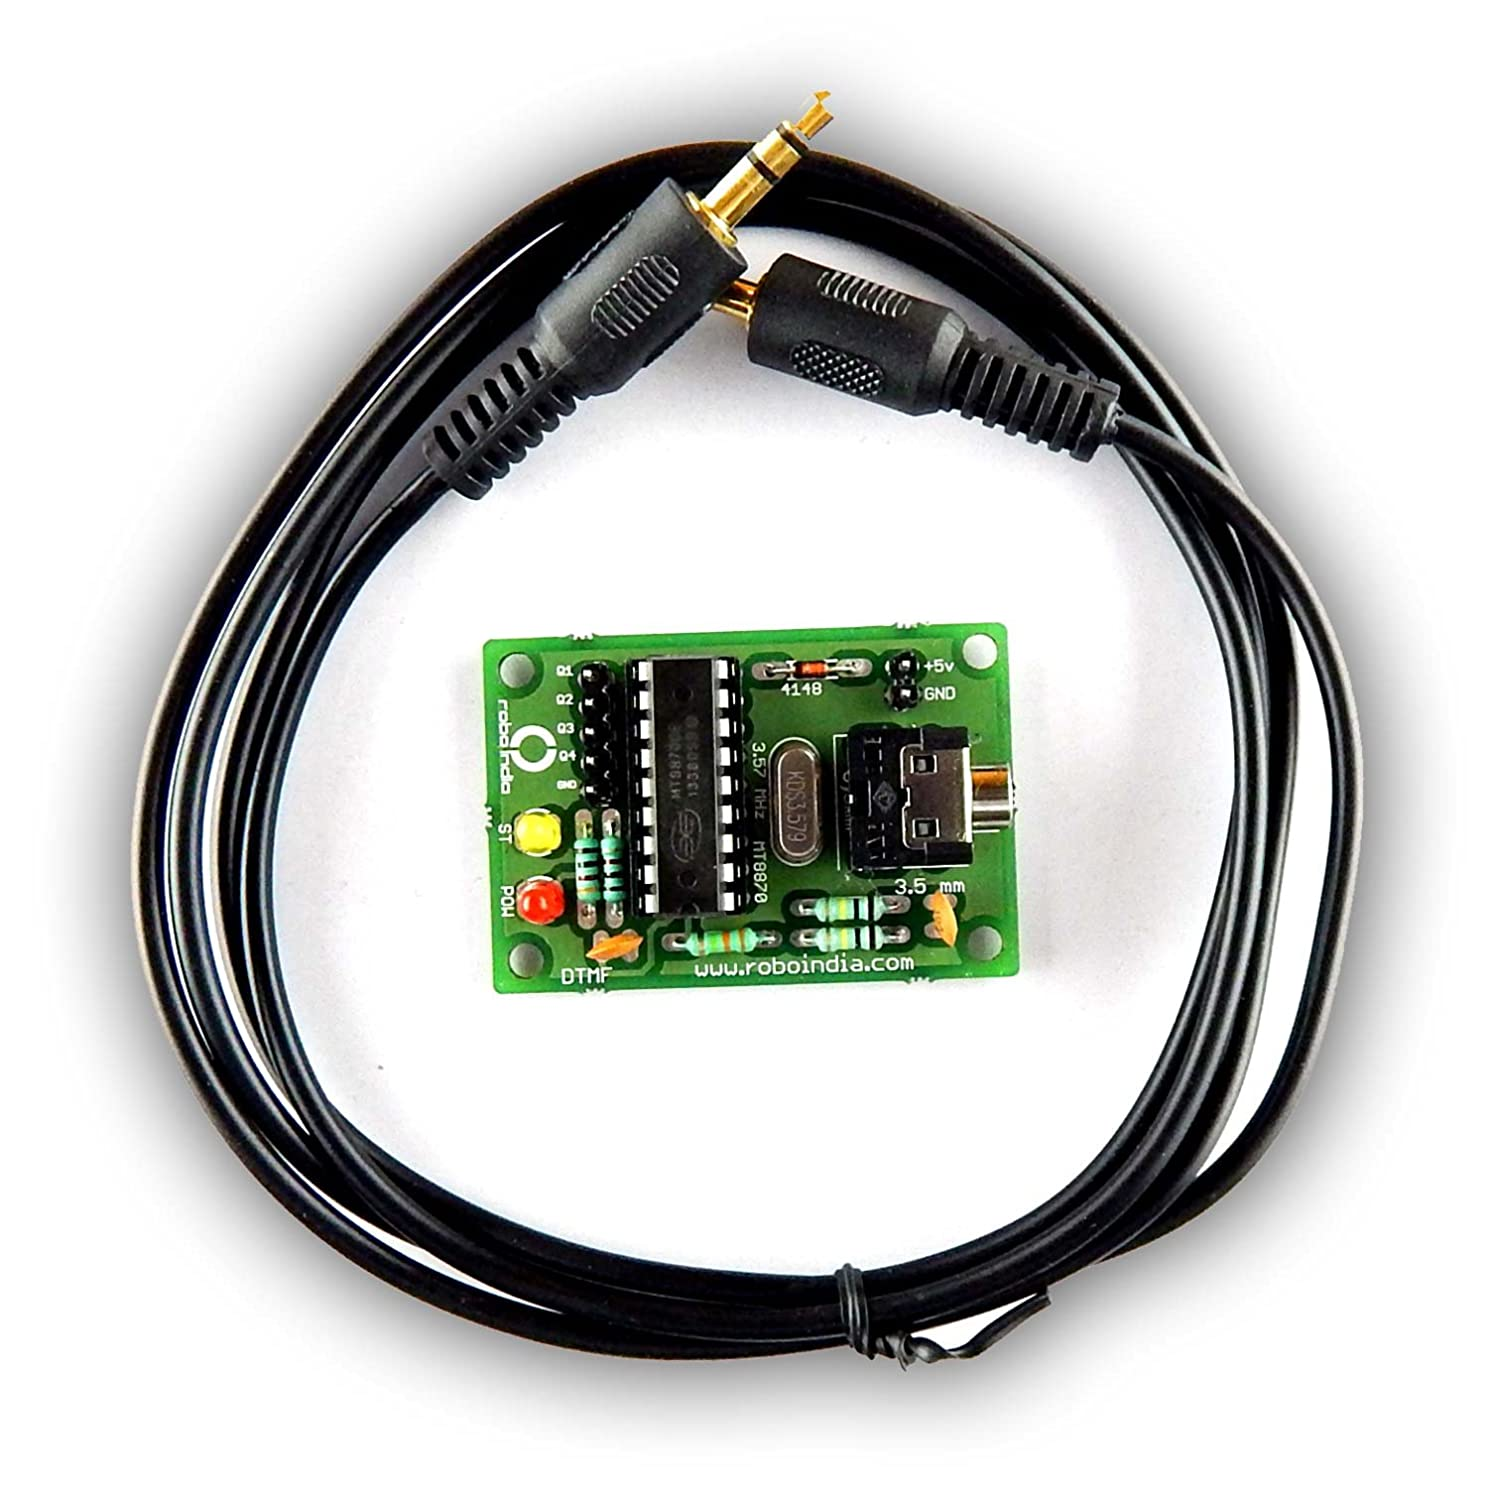
\includegraphics[width=3in]{Images/DTMF/DTMF_module.jpg}
    \caption[DTMF Module]{A \ac{DTMF} module }
    \setfloatalignment{b}
\end{figure}

\par The keypad is given a fixed set of pure tone ( pure sine wave ) that generates an audio of that particular frequency. This audio is analyzed at the switching centers and telephone equipment and decoded back to detect the key pressed. The keypad grid is divided into two groups of audio frequency ranges, The Row (Low group) frequencies and The Column (High group) frequencies. Whenever a key is pressed, corresponding mixture of audio are generated and transmitted via telephone line. Table ~\ref{fig:keypad} depicts how the frequency are distributed between rows and column.

\renewcommand{\arraystretch}{2.5}
\begin{table}
    \centering
    \begin{tabular}{|m{3em}|l|l|l|l|l|}
    \hline
         & \multicolumn{5}{c|}{Column(High Group) Frequencies}\\ \cline{2-6}
         &  & 1209 Hz & 1336Hz & 1477Hz & 1633Hz \\ \hline
        \multirow{4}{*}{\hspace{1.2mm} \rotatebox[origin=c]{90}{Row(Low Group)Frequencies}} & 697 Hz & 1 & 2 & 3 & A \\ \cline{2-6}
         & 770 Hz & 4 & 5 & 6 & B \\ \cline{2-6}
         & 852 Hz & 7 & 8 & 9 & C \\ \cline{2-6}
         & 941Hz & * & 0 & \# & D \\ \hline
    \end{tabular}
    \vspace{10mm}
    \caption[Keypad frequency]{Each key generates unique combination of frequency}
    \label{fig:keypad}
    \setfloatalignment{b}
\end{table}

%\begin{figure}
%    \centering
%    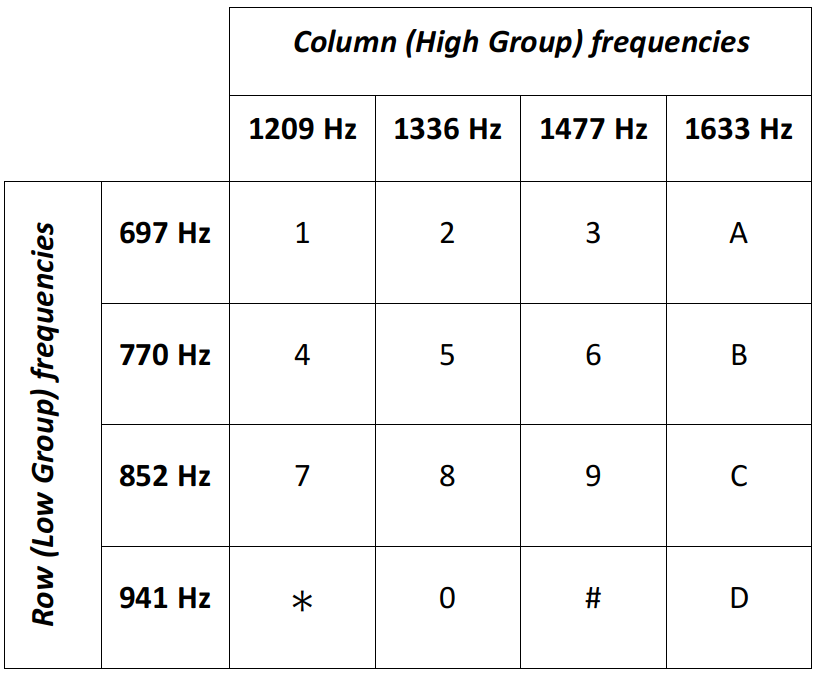
\includegraphics[width=4in]{Tables/DTMF/keypad_frequency.png}
%    \caption[Keypad frequency]{Each key generates unique combination of %frequency}
%    \label{fig:keypad}
%\end{figure}

\par For example if the customer presses 8 , audio of frequency 2188Hz (1336+852) is generated and transmitted via telephone line. At the receiving center, they are passed through a decoder to generate the key value 8.


\section{Number systems - Binary and Decimal}

\par In the digital world, number are represented in various forms. For humans to read smoothly, we in our day to day life make use of Decimal numbers. Decimal numbers have 10 possible digits, ranging from 0 to 9. All number are generated by placing these symbol in one’s, ten’s, hundred’s places. Notice that the places are represented as powers of 10. To remind that the number is in decimal system and not in some other system, we write 10 as its subscript. Since decimal numbers are the mostly used, its automatically assumed that the number is in decimal form, if there are no subscript written. Table \ref{fig:decimal} depicts few examples of decimal numbers.

\begin{figure}
    \centering
    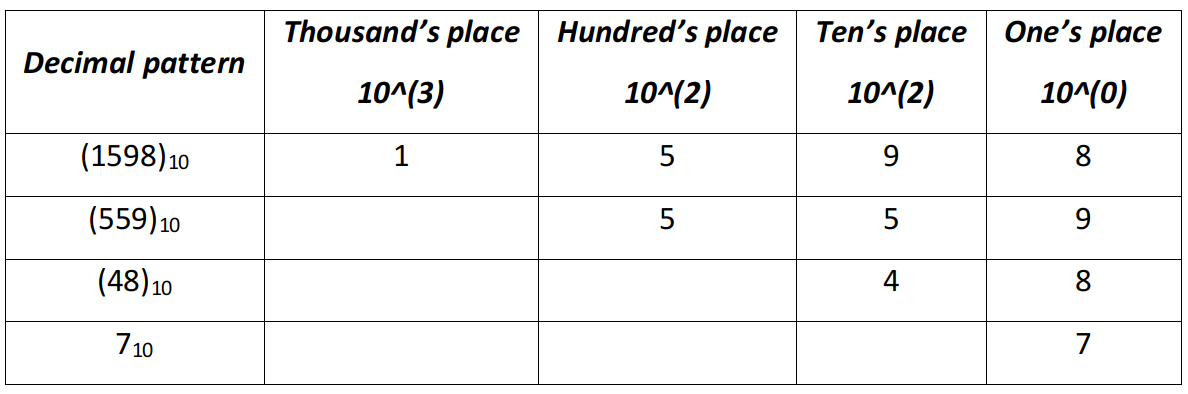
\includegraphics[width=4.3in]{Tables/DTMF/decimal_system.png}
    \caption[Decimal Number system]{Decimal number system}
    \label{fig:decimal}
\end{figure}

\par Consider a system that can accept N number of decimal digits (places) then, it means that the system can have $(base)^N$ possible values i.e., $10^N$ possible values ranging from 0 to $10^N - 1$ numbers. Assume we can accept any 4 digit decimal number. It means that there can be $10^4 = 10000$ values ranging from 0 to 9999 

\par Computers are digital systems where signal/states are represented by 0V or 5V. They have only 2 states possible. To execute any instruction, they require an array of 2 states called “bi-nary”. Each state are called as a bit. Bit zero represents 0V and bit one represents 5V. Hence to work upon decimal numbers, digital system needs to convert and represent decimal number as its equivalent binary numbers.

\par Consider a 3 bit binary number. There can be total of $2^3 = 8$ possible values, ranging from 0 to 7 as shown in the table \ref{fig:binary}.

\begin{figure}
    \centering
    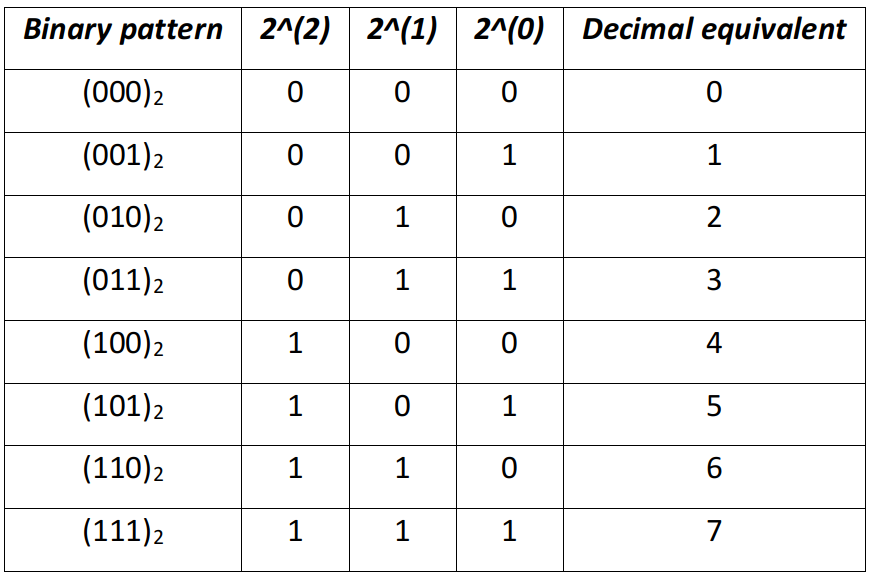
\includegraphics[width=4.3in]{Tables/DTMF/binary_system.png}
    \caption[Binary system]{A 3 bit binary to decimal mapping}
    \label{fig:binary}
\end{figure}

\par You might have heard of byte, kilo byte, megabyte etc. They denote range of collection of bits to represent an information. If “int” is 4 bytes long, it means it can have $24*8 = 232 = 4294967296$ possible values. See table \ref{fig:memory_size}

\begin{figure}
    \centering
    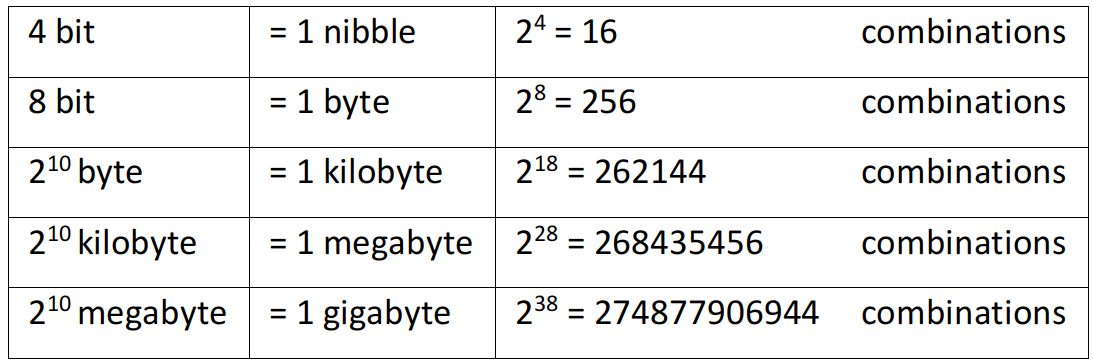
\includegraphics[width=4.3in]{Tables/DTMF/computer_memory.png}
    \caption[Memory size]{Computer memory capacity}
    \label{fig:memory_size}
\end{figure}

\section{Converting Decimal to Binary}

To convert a decimal number to its equivalent binary number, keep dividing the number by 2 and append the remainders in reverse order (bottom to top) as shown in figure \ref{fig:dec_to_bin}.

\begin{figure}
    \centering
    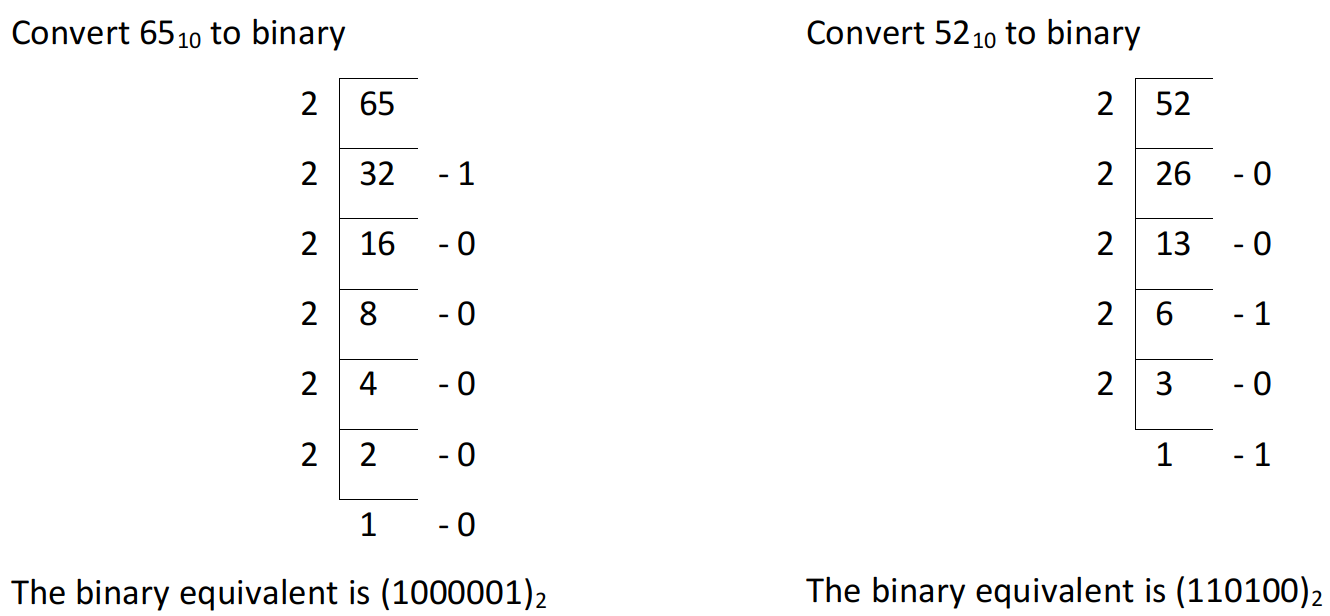
\includegraphics{Images/DTMF/decimal_to_binary.png}
    \caption[Decimal to binary]{Converting to binary}
    \label{fig:dec_to_bin}
\end{figure}

\section{Converting Binary to Decimal}

To convert binary number to its equivalent decimal number, keep multiplying the binary digit with $2^p$ , where p is digit position start from 0 and then find its sum as depicted in table \ref{fig:bin_to_dec}.

\begin{figure}
    \centering
    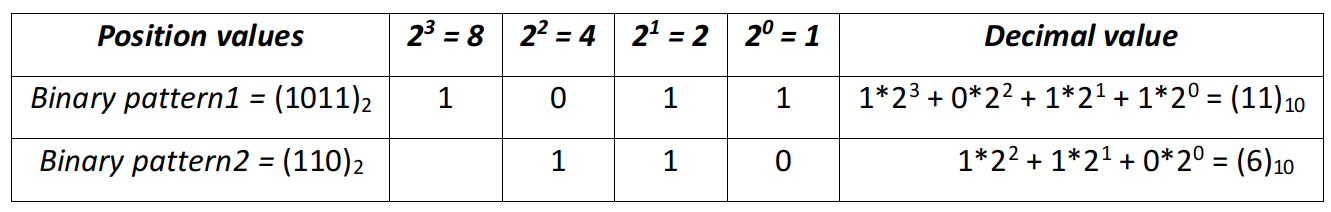
\includegraphics[width=4.3in]{Tables/DTMF/binary_decimal.png}
    \caption[Binary to decimal]{Converting to decimal}
    \label{fig:bin_to_dec}
\end{figure}

\section{MT8870 DTMF Decoder}

\ac{DTMF} decoder is a module the accepts the audio frequency and converts them to the digital signals. The audio can be fetched from a mobile phone via aux cable ( the headphone set) and connect it to the aux jack of the module. 

\begin{figure}
    \centering
    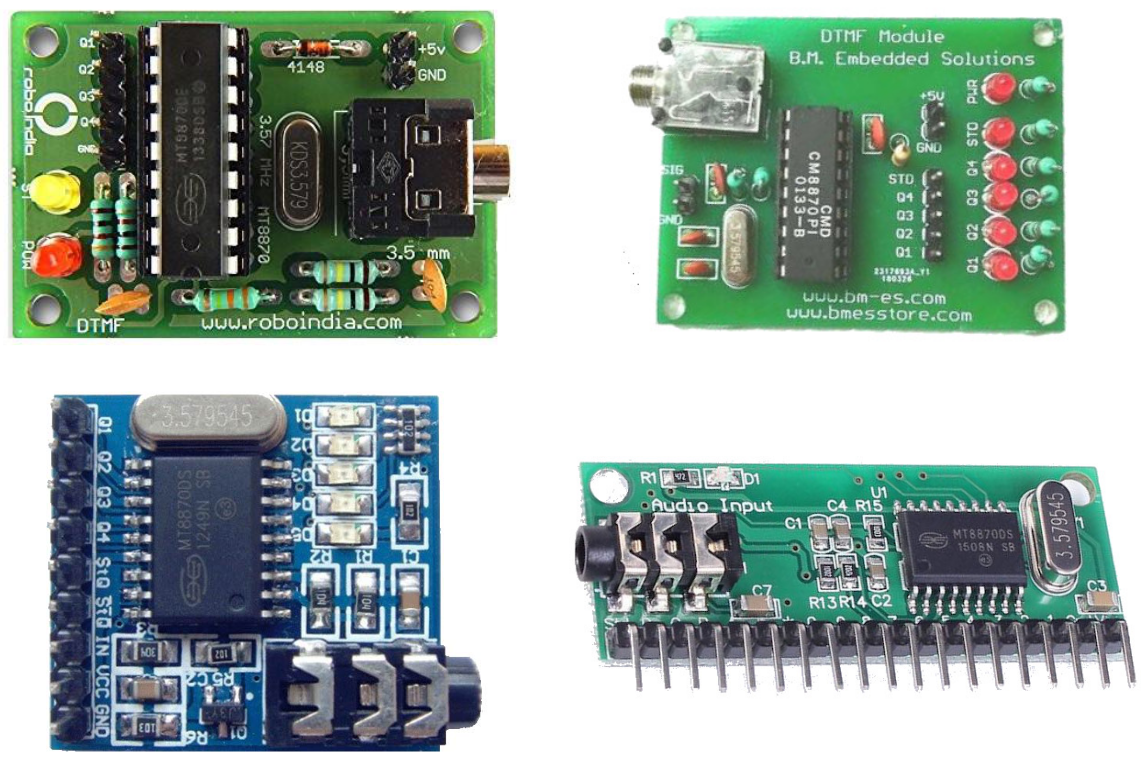
\includegraphics[width=4.3in]{Images/DTMF/DTMF_series.png}
    \caption[MT8870 DTMF decoder]{Various models of \ac{DTMF} decoder}
\end{figure}

\par The board needs to be powered up via 5V pins and the decoded output is received via pins Q1,Q2,Q3,Q4 in binary format. Table \ref{fig:dtmf_map} shows the mapping of key pressed from binary to decimal value.
\begin{figure}
    \centering
    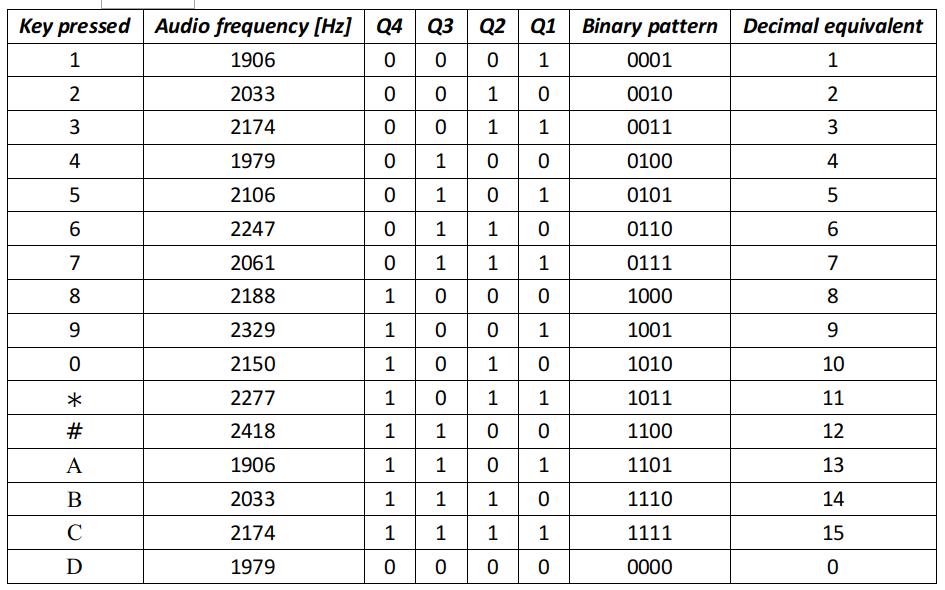
\includegraphics[width=4.3in]{Tables/DTMF/dtmf_pattern.png}
    \caption[DTMF pattern]{Mapping \ac{DTMF} inputs to decimal values}
    \label{fig:dtmf_map}
\end{figure}

\section{Programming DTMF decoder}
\begin{figure}
    \centering
    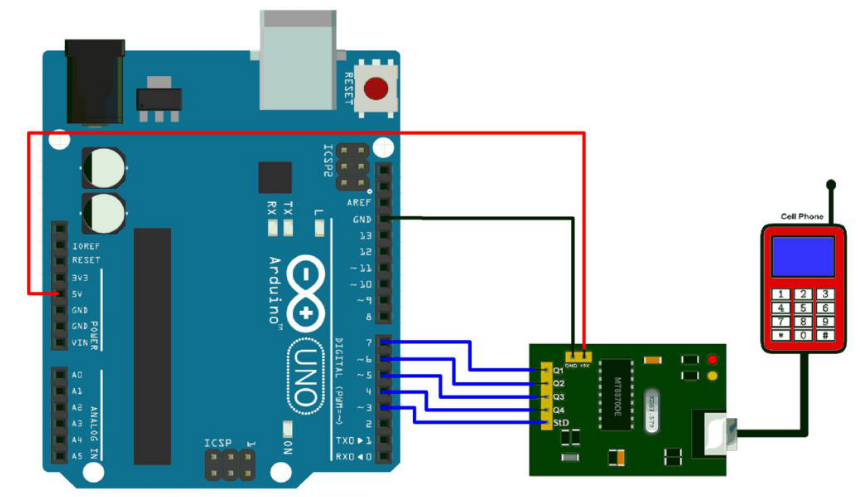
\includegraphics[width=4.3in]{Images/DTMF/DTMF_ckt.png}
    \caption[DTMF with Arduino]{Circuit diagram for interfacing \ac{DTMF} with Arduino Uno }
    \label{fig:dtmf_ckt}
\end{figure}

\par As shown in figure \ref{fig:dtmf_ckt}, the q1,q2,q3,q4 of \ac{DTMF} is connected to 7,6,5,4 pins of Arduino respectively. The StD pin is connected to pin3, which turns HIGH whenever the module receives a new frequency. The module is powered via 5V line and is connected to a cell phone via aux cable. The Phone acts as receiver/switch center. Lets write a code to interpret the \ac{DTMF} signals.
\vspace{0.2cm}
\begin{lstlisting}[style=CStyle]
int Q1=7, Q2=6, Q3=5, Q4=4, StD = 3; //pin allocations
int dec_number;

void setup(){
    //set pins as input for Arduino.
    pinMode(Q1,INPUT);pinMode(Q2,INPUT);
    pinMode(Q3,INPUT);pinMode(Q4,INPUT);
    pinMode(StD,INPUT);
    
    Serial.begin(9600);
}

void loop(){
    dec_number = 0;
    
    if(digitalRead(StD)==HIGH){ //received new frequency
    
        //converting binary signals to decimal number
        //using bit manipulation in C
        dec_number |= digitalRead(Q1)<<0 ;  //2^0 position
        dec_number |= digitalRead(Q2)<<1 ;	//2^1 position
        dec_number |= digitalRead(Q3)<<2 ;	//2^2 position
        dec_number |= digitalRead(Q4)<<3 ;	//2^3 position
        Serial.print("The code is "); 
        Serial.println(dec_number);
    }
}
\end{lstlisting}

\par Now make a call to the receiver phone \textbf{“A”} from another phone \textbf{“B”}. Make key presses in the phone B so that corresponding audio is heard at the phone A. Observe the Serial monitor for the output. It might happen that you cannot observe proper detection in the Serial monitor. This can be due to various factor like different audio jack material, internal phone circuitry, phone model and version etc. Try with some other phones. Have you ever noticed that whenever we press the button on earphone mic, it behaves differently in different phones?

\par Can you reconfigure the system to control a bot? Go through the section \ref{section:bot_interface} to get an idea to integrate the bot with \ac{DTMF}. Your wireless bot is ready for action.

\begin{figure}
	\centering
	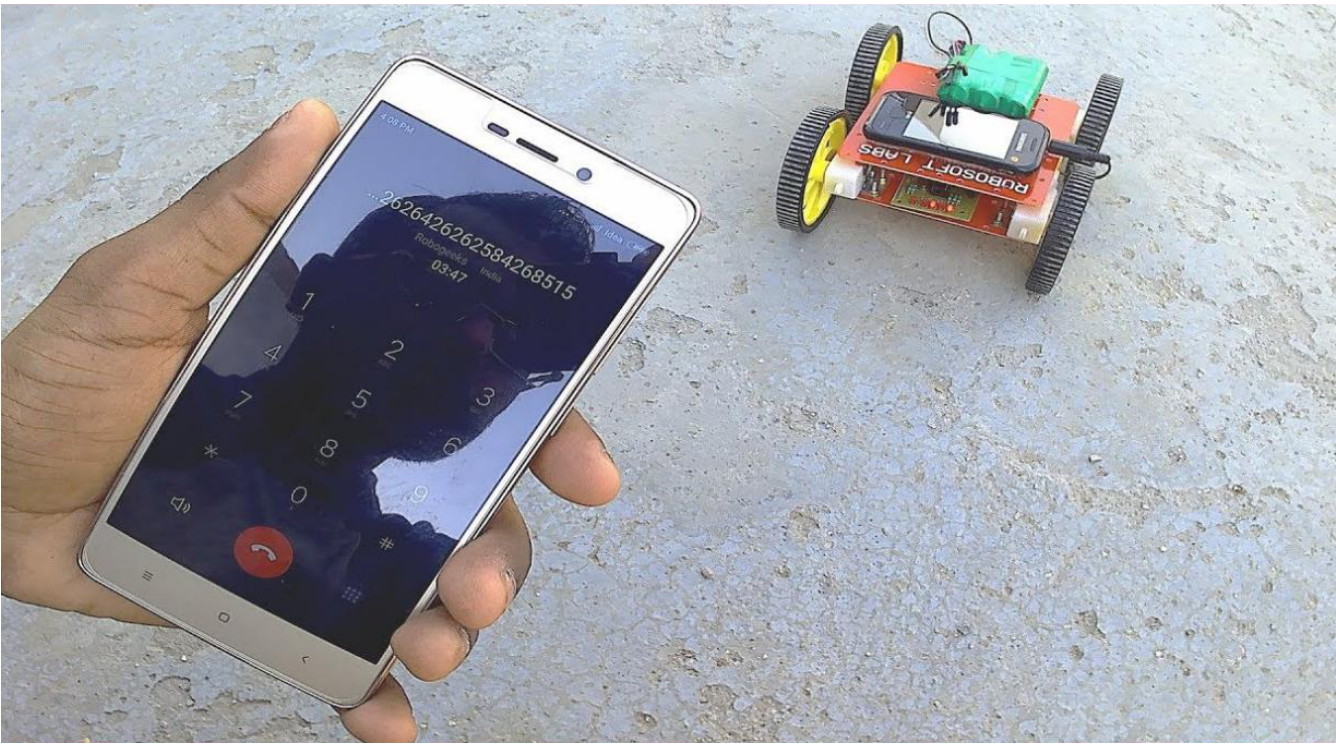
\includegraphics[width=4.3in]{Images/DTMF/wireless_bot.png}
\end{figure}

